% !TEX encoding = UTF-8 Unicode
% 予備審査レジュメ 11/26 作り直し(先生の指摘:結果をグラフで・表の書き方・囲いなし/あり・流れ)。前の版は resumeA_2p.tex。前の版は resume.tex(4 ページ)・resume2.tex(2 ページ)
% 図をページ幅で入れるため multicols ではなく twocolumn にした(11/22)
% ヘッダーは先輩(2025年度 7307)の「創造工学専攻 情報工学コース / 年度 特別研究 2 審査会」に合わせた
% ビルド:thesis/resume/ で latexmk resume.tex → build/resume.pdf
\documentclass[10pt,uplatex,dvipdfmx,twocolumn]{jsarticle}

% 描画・色関連
\usepackage[dvipdfmx]{graphicx}
\usepackage[dvipdfmx]{xcolor}
\usepackage{here}

% レイアウト調整関連
\usepackage{geometry}
\usepackage{setspace}
\usepackage{fancyhdr}
\usepackage{float}

% 数式関連
\usepackage{amsmath}
\usepackage{amssymb}
\usepackage{mathtools}
\usepackage{bm}

% 表・リスト関連
\usepackage{booktabs}
\usepackage{enumerate}

% テキスト装飾関連
\usepackage{url}

% キャプション関連
\usepackage{caption}
\usepackage{subcaption}

\graphicspath{{figures/}{../figures/}{../../experiments/}}
\geometry{a4paper, left=20mm,right=20mm,top=20mm,bottom=20mm}

\definecolor{tmcitblue}{cmyk}{0.86,0.91,0,0.04}
\pagestyle{fancy}
\fancyhf{}
\lhead{\color{tmcitblue}\footnotesize 東京都立産業技術高等専門学校}
\rhead{\color{tmcitblue}\footnotesize 専攻科 情報工学コース\\2026 年度特別研究Ⅱ予備審査会}
\lfoot{\color{tmcitblue}\footnotesize Tokyo Metropolitan College of Industrial Technology}
\cfoot{\thepage}
\renewcommand{\headrulewidth}{0.0pt}
\setlength{\headheight}{20.2781pt}
% ページ幅の図(figure*)をページの上に2つまで置けるように
\setcounter{dbltopnumber}{3}
\renewcommand{\dbltopfraction}{0.85}
\renewcommand{\dblfloatpagefraction}{0.85}
\renewcommand{\textfraction}{0.1}

% 節と図の前後の空きを詰める
\setlength{\textfloatsep}{8pt plus 2pt minus 2pt}
\setlength{\dbltextfloatsep}{8pt plus 2pt minus 2pt}
\captionsetup{skip=4pt}
\makeatletter
\renewcommand{\section}{\@startsection{section}{1}{\z@}{0.6\Cvs \@plus.3\Cdp}{0.3\Cvs}{\normalfont\large\headfont\raggedright}}
\renewcommand{\subsection}{\@startsection{subsection}{2}{\z@}{0.3\Cvs \@plus.2\Cdp}{0.1\Cvs}{\normalfont\normalsize\headfont}}
\makeatother

\begin{document}
\setstretch{1.00}
\twocolumn[{%
\centering
\Large{エッジマイクロクラスタにおける空間熱干渉を考慮した熱抑制手法の研究}\\
\vspace{6pt}
\large{7303 鈴木黎映}\\
\large{指導教員 知念賢一教授}
\vspace{10pt}
}]
% 赤字【】は結果待ち・要確認
\newcommand{\TBD}[1]{\textcolor{red}{【#1】}}

\section{はじめに}
データセンタでは、サーバの排熱が別のサーバの吸気側に回り込む熱の再循環が冷却の効率を下げる~\cite{moore,tang}。同じことは、小型の計算機を密に並べたエッジのマイクロクラスタ~\cite{iridis}でも起こりうる。あるノードの発熱で、ほかのノードの温度が上がる現象を、本研究では空間熱干渉と呼ぶ。Raspberry Pi 4B(以下、Raspi)は CPU 温度が約 80\,℃ を超えるとクロックを下げ(スロットリング)、処理が遅くなる。ファンを常に回せば温度は下がるが、ファンの寿命は稼働時間で表され~\cite{kim}、騒音にもなる。そのため、スロットリングを避けつつ、ファンの稼働をできるだけ減らしたい。

対外発表~\cite{ipsj}では、空間熱干渉を外部熱影響 $H$ として推定するカルマンフィルタを提案した。そこでは、密閉した容器の中で、隣のノードの負荷だけでアイドルのノードが約 12\,℃ 上がった。一方、開いたラックに横に並べた予備的な測定では 0.5\,℃ 未満であった。空間熱干渉は配置によって大きく変わるが、どのような配置で起こるのかは測られていなかった。温度を予測して先回りする熱管理~\cite{coskun,yeo}も、1 台の内部が対象である。そこで本研究では、同じ実機で次の 3 つを順に確かめる。
\begin{enumerate}
  \setlength{\itemsep}{0pt}
  \item[Q1] 空間熱干渉は、どの位置関係・囲いで起こるか
  \item[Q2] 干渉を $H$ として推定すると、温度の予測は当たるか
  \item[Q3] その予測でファンを制御すると、80\,℃ を超えずにファンの稼働を減らせるか
\end{enumerate}

\section{提案手法}
温度を室温からの上昇分 $\theta_t = T_t - T_{\mathrm{amb}}$ で表し、熱 RC モデルを 5 秒ごとに離散化する。
\begin{gather}
  \theta_{t+1} = a\,\theta_t + b\,u_t + c\,H_t + e\,f_t + d \\
  H_{t+1} = \rho\,H_t + (1-\rho)\,z_t
\end{gather}
$u_t$ は CPU 使用率、$f_t$ はファンの状態(0/1)、$z_t$ は周りのノードの温度の平均の基準からの変化分である。$b > 0$ は負荷による加熱、$e < 0$ はファンによる冷却、$c \ge 0$ は外部熱影響 $H_t$ の効きを表す。$[\theta_t, H_t]^\top$ をカルマンフィルタで推定し、今の負荷が続きファンは OFF のままと仮定して、30 秒先の温度と標準偏差 $\sigma_t$ を予測する。
\begin{equation}
  M_t = \alpha\,\sigma_t + \delta,\qquad T_{\mathrm{safe}} = T_{\mathrm{limit}} - M_t
\end{equation}
$\alpha = 2$、$\delta = 0.5$\,℃、$T_{\mathrm{limit}} = 80$\,℃ とし、予測温度が $T_{\mathrm{safe}}$ を超えたらファンを ON にする(最小 ON 時間 30 秒、OFF は 1\,℃ のヒステリシス)。

\section{実験}
\begin{figure}[tb]
  \centering
  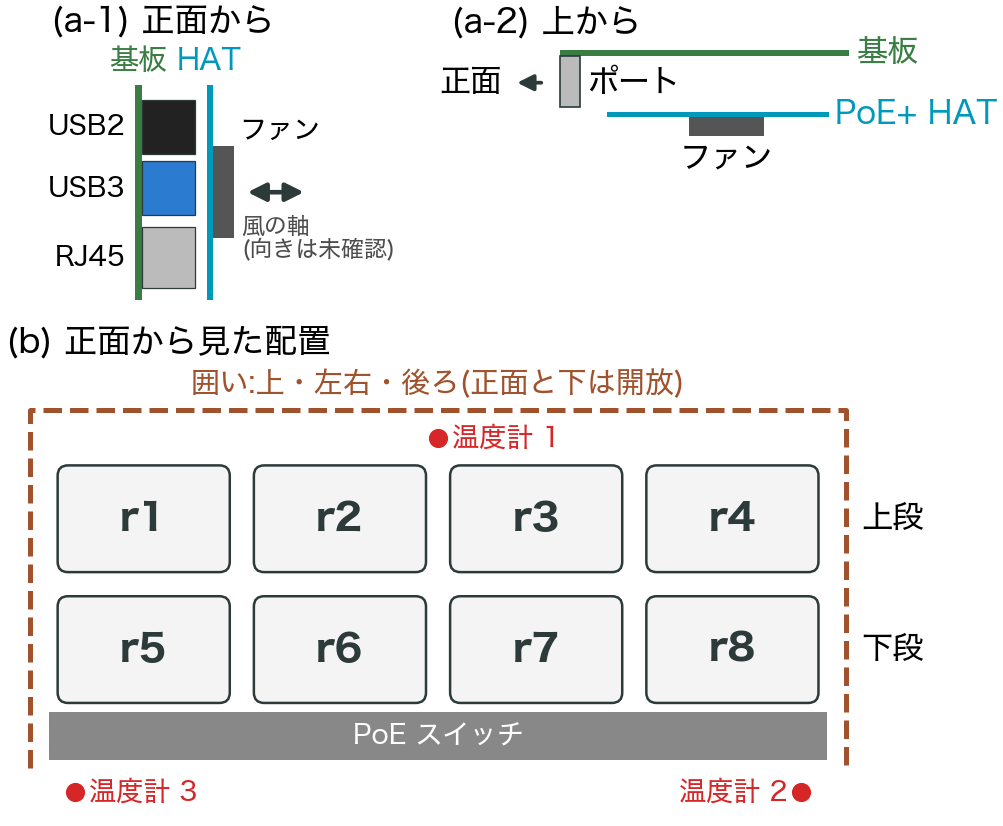
\includegraphics[width=\columnwidth]{fig_rack_layout.png}
  \caption{(a) 1 台の向き(8 台とも同じ)、(b) 配置}
  \label{fig:layout}
\end{figure}
Raspi 8 台を 10 インチラックに 2 段 × 4 列で、基板を立ててポートを正面に向けて取り付けた(図~\ref{fig:layout})。PoE+ HAT のファンは制御用 PC から ON/OFF し、止めている間は送風がなく自然対流だけになる。温度・CPU 使用率・クロック・ファンの状態を 1 秒ごとに、室温(囲いの外)と囲いの中の気温を約 1 分ごとに記録した。

囲いは「なし」と「あり」の 2 条件とした。囲いありは、ラック全体に段ボール箱(307 × 220 × 120\,mm、ラックの外形とほぼ同じ)をかぶせ、上・左右・後ろを覆い、正面と下を開けた。正面も閉じると負荷の前から箱の中が 40\,℃ に迫ったため、正面を開けた。

Q1 では、負荷を r6 だけ・r7 だけ・下段 4 台にかけ、負荷のないノードの上昇を測った。負荷は stress-ng で 2 コア 100\% を一度にかけ、10 分続けて 12 分休んだ。上昇は、負荷の最後 1 分と直前 1 分の平均温度の差から、同じ時間の室温の変化を引いた値とし、1\,℃ 以上を干渉ありとした。基準は測定の前に決めた。Q2 では、同じ実験の半分のデータで同定し、残りの半分で 30 秒先の予測を評価した。Q3 では、8 台に同じ 20 分の負荷パターン(0〜4 コア)を同時にかけ、常時 ON・しきい値(75\,℃ で ON、70\,℃ で OFF)・自ノードだけの予測・提案を比べた。

\section{結果}
\subsection{Q1:空間熱干渉はどこで起こるか}
\begin{figure}[tb]
  \centering
  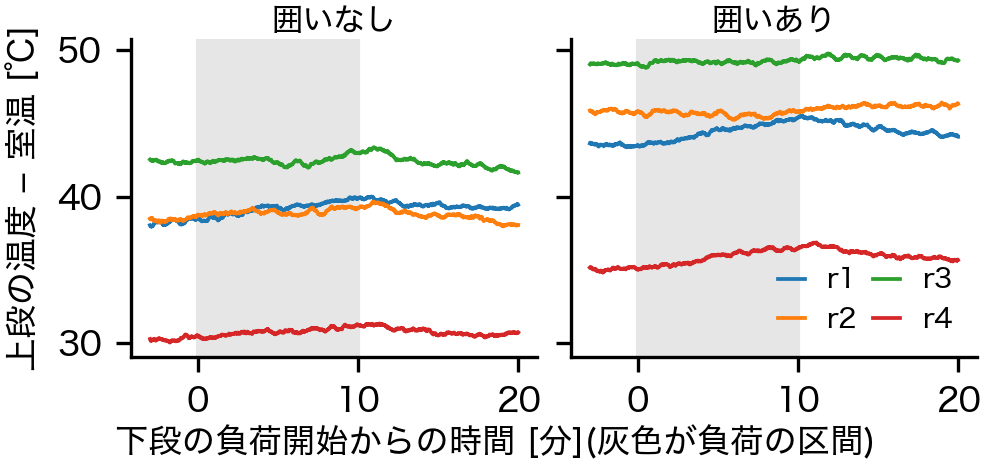
\includegraphics[width=\columnwidth]{fig_res_rise.png}
  \caption{下段に負荷をかけたときの上段の温度}
  \label{fig:rise}
\end{figure}
1 台だけに負荷をかけたとき、周りのノードの上昇は、囲いありでは真上・横・斜めのどれも $\pm 0.5$\,℃ 以内で、位置関係による差はなかった。囲いなしでは部屋の温度の揺れ(約 $\pm 1.5$\,℃)に埋もれた。一方、図~\ref{fig:rise}のように、囲いありでは負荷をかける前から上段の温度が 5〜10\,℃ 高く、下段 4 台に負荷をかけると上段の端(r1・r4)が 1.3〜1.8\,℃ 上がった。また、下段に 4 コアを 40 分かけ、下段のファンを回すと、上段は逆に 1〜2\,℃ 下がった。隣のファンの風が、囲いの中の空気を動かして周りも冷やしたためと考えられる。

\subsection{Q2:予測は当たるか}
\begin{figure}[tb]
  \centering
  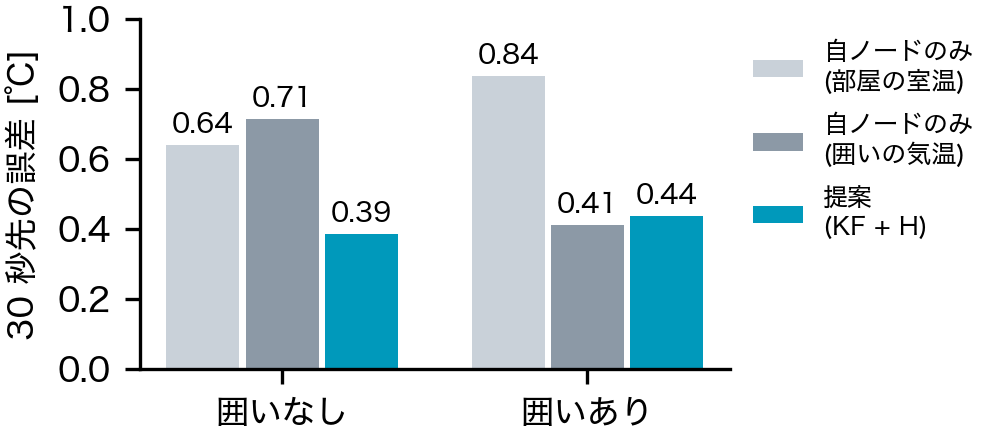
\includegraphics[width=\columnwidth]{fig_res_pred.png}
  \caption{30 秒先の予測の誤差(上段 r1〜r3 の平均)}
  \label{fig:pred}
\end{figure}
図~\ref{fig:pred}に、30 秒先の予測の平均絶対誤差を示す。提案(KF + $H$)は、部屋の室温だけを使う自ノードのモデルより、囲いなしで 0.64 から 0.39\,℃、囲いありで 0.84 から 0.44\,℃ に誤差を減らした。囲いありで提案が出した精度は、囲いの中に温度計を足して室温として使う自ノードのモデル(0.41\,℃)と同じで、提案はこれを追加の温度計なしで達成した。

\subsection{Q3:ファンの稼働を減らせるか}
\begin{figure}[tb]
  \centering
  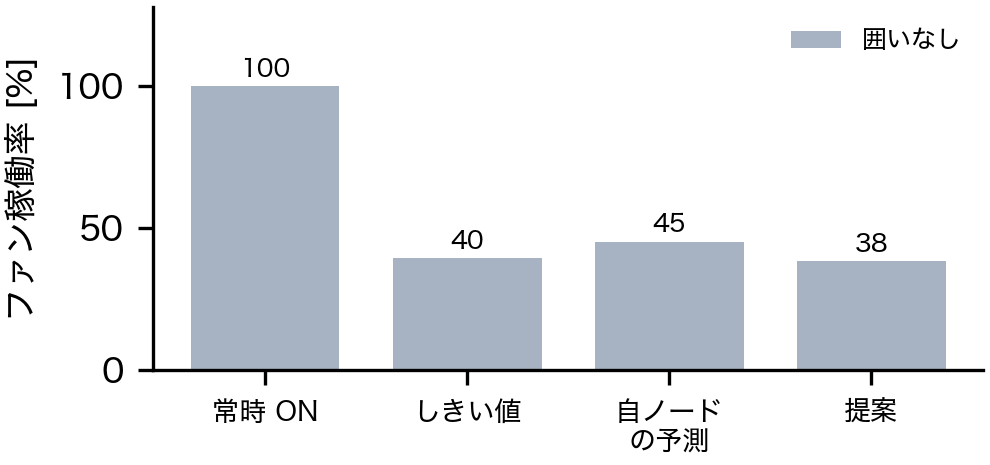
\includegraphics[width=\columnwidth]{fig_res_fan.png}
  \caption{方式ごとのファン稼働率}
  \label{fig:fan}
\end{figure}
図~\ref{fig:fan}に、20 分の負荷パターンでのファン稼働率を示す。囲いなし(3 台 × 3 巡)では、どの方式も 80\,℃ を超えず、提案は 38\% で常時 ON より約 6 割少なかったが、しきい値(40\%)との差はほぼなかった。囲いありでは、最初の比較で制御のモデルのファンの効きが 6 台で実測と合っておらず(ファン ON の温度を 10〜20\,℃ 低く見積もっていた)、同定し直して比較をやり直している。\TBD{囲いありの結果(段階 2 の弱いファン、11/26 午後)}

\section{考察とまとめ}
1 台の排熱が隣を直接温める経路は、囲いの有無・位置関係によらず 1\,℃ 未満であった。温度を押し上げていたのは囲いの中に熱が溜まる経路で、囲うだけで 5〜10\,℃ 高くなった。対外発表の約 12\,℃ も、密閉した容器で熱が溜まった結果と考えられる。隣のファンの風は周りを冷やす向きにも働いた。$H$ は、囲いの中に温度計がなくても、周りのノードの温度から囲いの昇温を推定でき、予測の誤差を約半分にした。一方、PoE+ HAT のファンは速く強いため、制御では予測としきい値の差が小さく、予測の利点は冷却の効きが遅い・弱い条件で出ると考えられる。今後は、ファンの段階を予測で選ぶ制御、ノードごとに負荷をずらした条件、負荷を徐々にかける条件で評価する。

\section*{対外発表}
本研究の手法の一部は、情報処理学会 OS 研究会で発表した~\cite{ipsj}。

\scriptsize{
\begin{thebibliography}{99}
  \setlength{\itemsep}{0pt}
  \bibitem{moore} J. Moore et al., ``Making Scheduling ``Cool'': Temperature-Aware Workload Placement in Data Centers,'' USENIX ATC, pp.61--74, 2005.
  \bibitem{tang} Q. Tang et al., ``Energy-Efficient Thermal-Aware Task Scheduling for Homogeneous HPC Data Centers,'' IEEE TPDS, Vol.19, No.11, pp.1458--1472, 2008.
  \bibitem{iridis} S. J. Cox et al., ``Iridis-pi: a low-cost, compact demonstration cluster,'' Cluster Computing, pp.349--358, 2014.
  \bibitem{kim} S. J. Kim, A. Claassen, ``How to Evaluate Fan Life,'' Electronics Cooling, 1996.
  \bibitem{ipsj} 鈴木 黎映, 知念 賢一, ``空間熱干渉を考慮した状態推定に基づく動的熱マージン制御手法,'' 情報処理学会研究報告, Vol.2026-OS-171, No.3, 2026.
  \bibitem{coskun} A. K. Coskun et al., ``Proactive Temperature Management in MPSoCs,'' Proc. ISLPED, 2008.
  \bibitem{yeo} I. Yeo et al., ``Predictive Dynamic Thermal Management for Multicore Systems,'' Proc. DAC, pp.734--739, 2008.
\end{thebibliography}
}
\end{document}
